\chapter{Hydrogen Atom}
\section{Fine Structure}
\subsection{Lamb Shift}
An interesting feature of the fine structure formula is that it depends only on $j$ and not $l$, moreover in general two different values of $l$ share the same energy. For example, the $2S_{}$ and $2P$ states should remain perfectly degenerate. However in 1947 Lamb and Retherford performed an experiment that displayed something to the contrary. The $S$ state is slightly higher in energy than the $p$ state. The explanation of this "Lamb" shift was later explained by Bethe, Feynman, Schwinger and Tomonaga (the founders of QED) as a corollary of the electromagnetic field itself being quantised.  Sharply in contrast to the hyperfine structure of Hydrogen, the Lamb shift is a completely novel i.e. non-classical (as the hyperfine structure is explained through Coulomb's law and the Biot-Savart Law) phenomena. It arises from a radiative correction in Quantum Electrodynamics to which classical theories are mute. In Feynman lingo, this arises from loop corrections as potrayed below.
\begin{figure}[h]
	\centering
	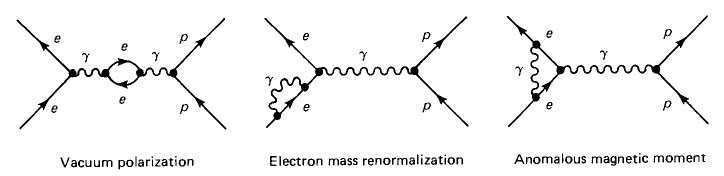
\includegraphics[width=0.6\linewidth, height=0.3\linewidth]{feyn-loop.png}
\end{figure}
Naively,
\begin{enumerate}
\item the first diagram describes pair-production in the neighbhorhood of a nucleus, leading to a partial screening effect of the proton's charge;
\item the second diagram reflects the fact that the electromagnetic field has a non-zero ground state
\item the third diagram leads to a tiny modification of the electron's magnetic dipole moment (an addition of $a + \alpha/2\pi = 1.00116$)
\end{enumerate}
We shall not discuss the results in depth but rather consider two exemplary cases:\\
For $ l = 0$,
\begin{equation}
	\Delta E_{Lamb} = \alpha^{5}mc^{2}\frac{1}{4n^{3}}\left[k(n,0)\right]
\end{equation}
Where $k(n,0)$ is a numerical factor defined as:
$$k(n,0) = \begin{cases}
12.7, & \text{if } n = 1\\
13.2,              & \text{if } n \rightarrow \infty
\end{cases} $$
For $ l = 0$ and $j = l \pm \frac{1}{2}$,
\begin{equation}
\Delta E_{Lamb} = \alpha^{5}mc^{2}\frac{1}{4n^{3}}\left[ k(n,0) \pm \frac{1}{\pi (l + \frac{1}{2}) (l + \frac{1}{2})} \right]
\end{equation}
Here, $k(n,l)$ is a very small number $(< 0.05)$ which varies a little with it's arguments.\\
The Lamb shift is tiny except for the case $l=0$, for which it amounts to about $10 \% $ of the fine structure. However, since it depends on $l$, it lifts the degeneracy of the pairs of states with common $n$ and $j$ and in particular it splits $2 S_{1/2}$ and $2 P_{1/2}$.
\section{The Zeeman Effect}
When an atom is placed in a uniform magnetic field $B_{Ext.}$, the energy levels are shifted, this is known as the Zeeman effect. For the case of a single electron, the shift is:
\begin{equation}
H^{'}_{Z} = -(\mu_{l} + \mu_{s}).B_{Ext.}
\end{equation}
Where,
\begin{equation}
content...
\end{equation}
is the magnetic dipole moment associated with electron spin, and
\begin{equation}
	content...
\end{equation}
is the dipole moment associated with orbital motion. The gyromagnetic ratio in this case is simply classical i.e. $q/2m$, it is only for spin that we have an extra factor of 2. We now rewrite () as:
\begin{equation}
asd
\end{equation}
The nature of the Zeeman splitting depnds on the strength of the external field vs. the internal one that gives rise to spin-orbit/spin-spin coupling. This table provides a short review of the different cases:
\begin{center}
\begin{tabularx}{0.9\textwidth} { 
		| >{\centering\arraybackslash}X 
		| >{\centering\arraybackslash}X 
		| >{\centering\arraybackslash}X | }
	\hline
	\textbf{Case} & \textbf{Name} & \textbf{Comments} \\
	\hline
	$B_{Ext.} >> B_{Int.}$  & Strong-Field Zeeman Effect  & Zeeman effect dominates; fine structure becomes the perturbation  \\
	\hline
	$B_{Ext.} << B_{Int.}$  & Weak-Field Zeeman Effect  & Fine structure dominates; $H^{'}_{z}$ can be treated as a small perturbation   \\
	\hline
	$B_{Ext.} = B_{Int.}$  & Intermediate Zeeman Effect  & Both the fields are equal in strength thus we would need elements of degenerate peturbation theory and will need to diagonlize the necessary portion of the Hamiltonian "by hand" \\
	\hline
\end{tabularx}
\end{center}
In the next few sections we'll explore all of them in depth.
\subsection{Weak-Field Zeeman Effect}
\subsection{Strong-Field Zeeman Effect}
\subsection{Intermediate Zeeman Effect}
\section{Hyperfine Splitting in Hydrogen}

